\chapter{The Deputy Procureur du Roi}

In one of the aristocratic mansions built by Puget in the Rue du Grand
Cours opposite the Medusa fountain, a second marriage feast was being
celebrated, almost at the same hour with the nuptial repast given by
Dantès. In this case, however, although the occasion of the
entertainment was similar, the company was strikingly dissimilar.
Instead of a rude mixture of sailors, soldiers, and those belonging to
the humblest grade of life, the present assembly was composed of the
very flower of Marseilles society,—magistrates who had resigned their
office during the usurper’s reign; officers who had deserted from the
imperial army and joined forces with Condé; and younger members of
families, brought up to hate and execrate the man whom five years of
exile would convert into a martyr, and fifteen of restoration elevate
to the rank of a god.

The guests were still at table, and the heated and energetic
conversation that prevailed betrayed the violent and vindictive
passions that then agitated each dweller of the South, where unhappily,
for five centuries religious strife had long given increased bitterness
to the violence of party feeling.

The emperor, now king of the petty Island of Elba, after having held
sovereign sway over one-half of the world, counting as his subjects a
small population of five or six thousand souls,—after having been
accustomed to hear the “\textit{Vive Napoléons}” of a hundred and twenty
millions of human beings, uttered in ten different languages,—was
looked upon here as a ruined man, separated forever from any fresh
connection with France or claim to her throne.

The magistrates freely discussed their political views; the military
part of the company talked unreservedly of Moscow and Leipsic, while
the women commented on the divorce of Josephine. It was not over the
downfall of the man, but over the defeat of the Napoleonic idea, that
they rejoiced, and in this they foresaw for themselves the bright and
cheering prospect of a revivified political existence.

An old man, decorated with the cross of Saint Louis, now rose and
proposed the health of King Louis XVIII. It was the Marquis de
Saint-Méran. This toast, recalling at once the patient exile of
Hartwell and the peace-loving King of France, excited universal
enthusiasm; glasses were elevated in the air \textit{à l’Anglaise}, and the
ladies, snatching their bouquets from their fair bosoms, strewed the
table with their floral treasures. In a word, an almost poetical fervor
prevailed.

“Ah,” said the Marquise de Saint-Méran, a woman with a stern,
forbidding eye, though still noble and distinguished in appearance,
despite her fifty years—“ah, these revolutionists, who have driven us
from those very possessions they afterwards purchased for a mere trifle
during the Reign of Terror, would be compelled to own, were they here,
that all true devotion was on our side, since we were content to follow
the fortunes of a falling monarch, while they, on the contrary, made
their fortune by worshipping the rising sun; yes, yes, they could not
help admitting that the king, for whom we sacrificed rank, wealth, and
station was truly our ‘Louis the well-beloved,’ while their wretched
usurper has been, and ever will be, to them their evil genius, their
‘Napoleon the accursed.’ Am I not right, Villefort?”

“I beg your pardon, madame. I really must pray you to excuse me, but—in
truth—I was not attending to the conversation.”

“Marquise, marquise!” interposed the old nobleman who had proposed the
toast, “let the young people alone; let me tell you, on one’s wedding
day there are more agreeable subjects of conversation than dry
politics.”

“Never mind, dearest mother,” said a young and lovely girl, with a
profusion of light brown hair, and eyes that seemed to float in liquid
crystal, “’tis all my fault for seizing upon M. de Villefort, so as to
prevent his listening to what you said. But there—now take him—he is
your own for as long as you like. M. Villefort, I beg to remind you my
mother speaks to you.”

“If the marquise will deign to repeat the words I but imperfectly
caught, I shall be delighted to answer,” said M. de Villefort.

“Never mind, Renée,” replied the marquise, with a look of tenderness
that seemed out of keeping with her harsh dry features; but, however
all other feelings may be withered in a woman’s nature, there is always
one bright smiling spot in the desert of her heart, and that is the
shrine of maternal love. “I forgive you. What I was saying, Villefort,
was, that the Bonapartists had not our sincerity, enthusiasm, or
devotion.”

“They had, however, what supplied the place of those fine qualities,”
replied the young man, “and that was fanaticism. Napoleon is the
Mahomet of the West, and is worshipped by his commonplace but ambitious
followers, not only as a leader and lawgiver, but also as the
personification of equality.”

“He!” cried the marquise: “Napoleon the type of equality! For mercy’s
sake, then, what would you call Robespierre? Come, come, do not strip
the latter of his just rights to bestow them on the Corsican, who, to
my mind, has usurped quite enough.”

\begin{figure}[h]
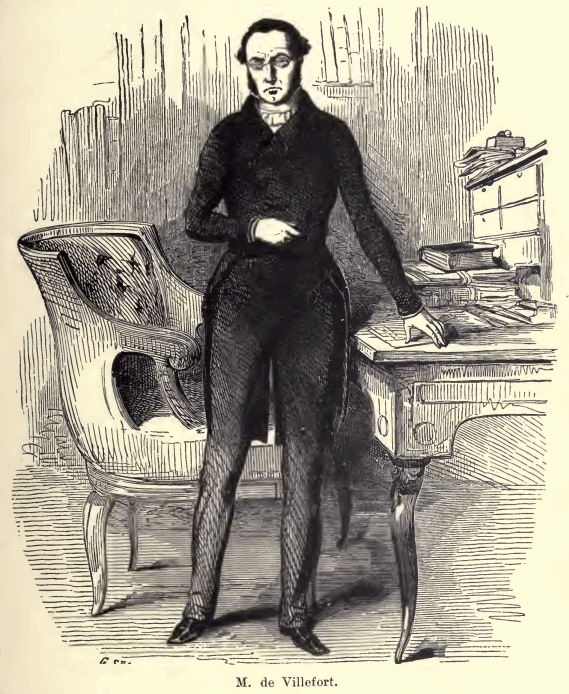
\includegraphics[width=\textwidth]{0085m.jpg}
\end{figure}

“Nay, madame; I would place each of these heroes on his right
pedestal—that of Robespierre on his scaffold in the Place Louis Quinze;
that of Napoleon on the column of the Place Vendôme. The only
difference consists in the opposite character of the equality advocated
by these two men; one is the equality that elevates, the other is the
equality that degrades; one brings a king within reach of the
guillotine, the other elevates the people to a level with the throne.
Observe,” said Villefort, smiling, “I do not mean to deny that both
these men were revolutionary scoundrels, and that the 9th Thermidor and
the 4th of April, in the year 1814, were lucky days for France, worthy
of being gratefully remembered by every friend to monarchy and civil
order; and that explains how it comes to pass that, fallen, as I trust
he is forever, Napoleon has still retained a train of parasitical
satellites. Still, marquise, it has been so with other
usurpers—Cromwell, for instance, who was not half so bad as Napoleon,
had his partisans and advocates.”

“Do you know, Villefort, that you are talking in a most dreadfully
revolutionary strain? But I excuse it, it is impossible to expect the
son of a Girondin to be free from a small spice of the old leaven.” A
deep crimson suffused the countenance of Villefort.

“’Tis true, madame,” answered he, “that my father was a Girondin, but
he was not among the number of those who voted for the king’s death; he
was an equal sufferer with yourself during the Reign of Terror, and had
well-nigh lost his head on the same scaffold on which your father
perished.”

“True,” replied the marquise, without wincing in the slightest degree
at the tragic remembrance thus called up; “but bear in mind, if you
please, that our respective parents underwent persecution and
proscription from diametrically opposite principles; in proof of which
I may remark, that while my family remained among the staunchest
adherents of the exiled princes, your father lost no time in joining
the new government; and that while the Citizen Noirtier was a Girondin,
the Count Noirtier became a senator.”

“Dear mother,” interposed Renée, “you know very well it was agreed that
all these disagreeable reminiscences should forever be laid aside.”

“Suffer me, also, madame,” replied Villefort, “to add my earnest
request to Mademoiselle de Saint-Méran’s, that you will kindly allow
the veil of oblivion to cover and conceal the past. What avails
recrimination over matters wholly past recall? For my own part, I have
laid aside even the name of my father, and altogether disown his
political principles. He was—nay, probably may still be—a Bonapartist,
and is called Noirtier; I, on the contrary, am a staunch royalist, and
style myself de Villefort. Let what may remain of revolutionary sap
exhaust itself and die away with the old trunk, and condescend only to
regard the young shoot which has started up at a distance from the
parent tree, without having the power, any more than the wish, to
separate entirely from the stock from which it sprung.”

“Bravo, Villefort!” cried the marquis; “excellently well said! Come,
now, I have hopes of obtaining what I have been for years endeavoring
to persuade the marquise to promise; namely, a perfect amnesty and
forgetfulness of the past.”

“With all my heart,” replied the marquise; “let the past be forever
forgotten. I promise you it affords \textit{me} as little pleasure to revive
it as it does you. All I ask is, that Villefort will be firm and
inflexible for the future in his political principles. Remember, also,
Villefort, that we have pledged ourselves to his majesty for your
fealty and strict loyalty, and that at our recommendation the king
consented to forget the past, as I do” (and here she extended to him
her hand)—“as I now do at your entreaty. But bear in mind, that should
there fall in your way anyone guilty of conspiring against the
government, you will be so much the more bound to visit the offence
with rigorous punishment, as it is known you belong to a suspected
family.”

“Alas, madame,” returned Villefort, “my profession, as well as the
times in which we live, compels me to be severe. I have already
successfully conducted several public prosecutions, and brought the
offenders to merited punishment. But we have not done with the thing
yet.”

\begin{figure}[ht]
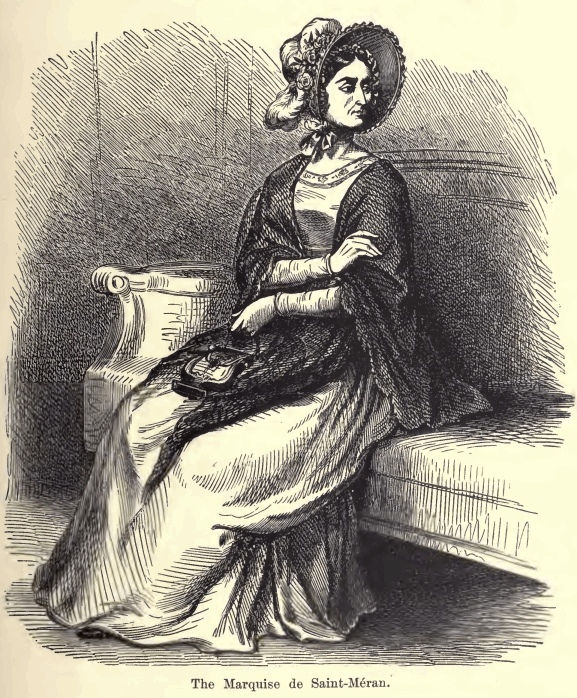
\includegraphics[width=\textwidth]{0087m.jpg}
\end{figure}

“Do you, indeed, think so?” inquired the marquise.

“I am, at least, fearful of it. Napoleon, in the Island of Elba, is too
near France, and his proximity keeps up the hopes of his partisans.
Marseilles is filled with half-pay officers, who are daily, under one
frivolous pretext or other, getting up quarrels with the royalists;
from hence arise continual and fatal duels among the higher classes of
persons, and assassinations in the lower.”

“You have heard, perhaps,” said the Comte de Salvieux, one of M. de
Saint-Méran’s oldest friends, and chamberlain to the Comte d’Artois,
“that the Holy Alliance purpose removing him from thence?”

“Yes; they were talking about it when we left Paris,” said M. de
Saint-Méran; “and where is it decided to transfer him?”

“To Saint Helena.”

“For heaven’s sake, where is that?” asked the marquise.

“An island situated on the other side of the equator, at least two
thousand leagues from here,” replied the count.

“So much the better. As Villefort observes, it is a great act of folly
to have left such a man between Corsica, where he was born, and Naples,
of which his brother-in-law is king, and face to face with Italy, the
sovereignty of which he coveted for his son.”

“Unfortunately,” said Villefort, “there are the treaties of 1814, and
we cannot molest Napoleon without breaking those compacts.”

“Oh, well, we shall find some way out of it,” responded M. de Salvieux.
“There wasn’t any trouble over treaties when it was a question of
shooting the poor Duc d’Enghien.”

“Well,” said the marquise, “it seems probable that, by the aid of the
Holy Alliance, we shall be rid of Napoleon; and we must trust to the
vigilance of M. de Villefort to purify Marseilles of his partisans. The
king is either a king or no king; if he be acknowledged as sovereign of
France, he should be upheld in peace and tranquillity; and this can
best be effected by employing the most inflexible agents to put down
every attempt at conspiracy—’tis the best and surest means of
preventing mischief.”

“Unfortunately, madame,” answered Villefort, “the strong arm of the law
is not called upon to interfere until the evil has taken place.”

“Then all he has got to do is to endeavor to repair it.”

“Nay, madame, the law is frequently powerless to effect this; all it
can do is to avenge the wrong done.”

“Oh, M. de Villefort,” cried a beautiful young creature, daughter to
the Comte de Salvieux, and the cherished friend of Mademoiselle de
Saint-Méran, “do try and get up some famous trial while we are at
Marseilles. I never was in a law-court; I am told it is so very
amusing!”

“Amusing, certainly,” replied the young man, “inasmuch as, instead of
shedding tears as at the fictitious tale of woe produced at a theatre,
you behold in a law-court a case of real and genuine distress—a drama
of life. The prisoner whom you there see pale, agitated, and alarmed,
instead of—as is the case when a curtain falls on a tragedy—going home
to sup peacefully with his family, and then retiring to rest, that he
may recommence his mimic woes on the morrow,—is removed from your sight
merely to be reconducted to his prison and delivered up to the
executioner. I leave you to judge how far your nerves are calculated to
bear you through such a scene. Of this, however, be assured, that
should any favorable opportunity present itself, I will not fail to
offer you the choice of being present.”

“For shame, M. de Villefort!” said Renée, becoming quite pale; “don’t
you see how you are frightening us?—and yet you laugh.”

“What would you have? ’Tis like a duel. I have already recorded
sentence of death, five or six times, against the movers of political
conspiracies, and who can say how many daggers may be ready sharpened,
and only waiting a favorable opportunity to be buried in my heart?”

“Gracious heavens, M. de Villefort,” said Renée, becoming more and more
terrified; “you surely are not in earnest.”

“Indeed I am,” replied the young magistrate with a smile; “and in the
interesting trial that young lady is anxious to witness, the case would
only be still more aggravated. Suppose, for instance, the prisoner, as
is more than probable, to have served under Napoleon—well, can you
expect for an instant, that one accustomed, at the word of his
commander, to rush fearlessly on the very bayonets of his foe, will
scruple more to drive a stiletto into the heart of one he knows to be
his personal enemy, than to slaughter his fellow-creatures, merely
because bidden to do so by one he is bound to obey? Besides, one
requires the excitement of being hateful in the eyes of the accused, in
order to lash one’s self into a state of sufficient vehemence and
power. I would not choose to see the man against whom I pleaded smile,
as though in mockery of my words. No; my pride is to see the accused
pale, agitated, and as though beaten out of all composure by the fire
of my eloquence.” Renée uttered a smothered exclamation.

“Bravo!” cried one of the guests; “that is what I call talking to some
purpose.”

“Just the person we require at a time like the present,” said a second.

“What a splendid business that last case of yours was, my dear
Villefort!” remarked a third; “I mean the trial of the man for
murdering his father. Upon my word, you killed him ere the executioner
had laid his hand upon him.”

“Oh, as for parricides, and such dreadful people as that,” interposed
Renée, “it matters very little what is done to them; but as regards
poor unfortunate creatures whose only crime consists in having mixed
themselves up in political intrigues——”

“Why, that is the very worst offence they could possibly commit; for,
don’t you see, Renée, the king is the father of his people, and he who
shall plot or contrive aught against the life and safety of the parent
of thirty-two millions of souls, is a parricide upon a fearfully great
scale?”

“I don’t know anything about that,” replied Renée; “but, M. de
Villefort, you have promised me—have you not?—always to show mercy to
those I plead for.”

“Make yourself quite easy on that point,” answered Villefort, with one
of his sweetest smiles; “you and I will always consult upon our
verdicts.”

“My love,” said the marquise, “attend to your doves, your lap-dogs, and
embroidery, but do not meddle with what you do not understand. Nowadays
the military profession is in abeyance and the magisterial robe is the
badge of honor. There is a wise Latin proverb that is very much in
point.”

“\textit{Cedant arma togæ},” said Villefort with a bow.

“I cannot speak Latin,” responded the marquise.

“Well,” said Renée, “I cannot help regretting you had not chosen some
other profession than your own—a physician, for instance. Do you know I
always felt a shudder at the idea of even a \textit{destroying} angel?”

“Dear, good Renée,” whispered Villefort, as he gazed with unutterable
tenderness on the lovely speaker.

“Let us hope, my child,” cried the marquis, “that M. de Villefort may
prove the moral and political physician of this province; if so, he
will have achieved a noble work.”

“And one which will go far to efface the recollection of his father’s
conduct,” added the incorrigible marquise.

“Madame,” replied Villefort, with a mournful smile, “I have already had
the honor to observe that my father has—at least, I hope so—abjured his
past errors, and that he is, at the present moment, a firm and zealous
friend to religion and order—a better royalist, possibly, than his son;
for he has to atone for past dereliction, while I have no other impulse
than warm, decided preference and conviction.” Having made this
well-turned speech, Villefort looked carefully around to mark the
effect of his oratory, much as he would have done had he been
addressing the bench in open court.

“Do you know, my dear Villefort,” cried the Comte de Salvieux, “that is
exactly what I myself said the other day at the Tuileries, when
questioned by his majesty’s principal chamberlain touching the
singularity of an alliance between the son of a Girondin and the
daughter of an officer of the Duc de Condé; and I assure you he seemed
fully to comprehend that this mode of reconciling political differences
was based upon sound and excellent principles. Then the king, who,
without our suspecting it, had overheard our conversation, interrupted
us by saying, ‘Villefort’—observe that the king did not pronounce the
word Noirtier, but, on the contrary, placed considerable emphasis on
that of Villefort—‘Villefort,’ said his majesty, ‘is a young man of
great judgment and discretion, who will be sure to make a figure in his
profession; I like him much, and it gave me great pleasure to hear that
he was about to become the son-in-law of the Marquis and Marquise de
Saint-Méran. I should myself have recommended the match, had not the
noble marquis anticipated my wishes by requesting my consent to it.’”

“Is it possible the king could have condescended so far as to express
himself so favorably of me?” asked the enraptured Villefort.

“I give you his very words; and if the marquis chooses to be candid, he
will confess that they perfectly agree with what his majesty said to
him, when he went six months ago to consult him upon the subject of
your espousing his daughter.”

\begin{figure}[ht]
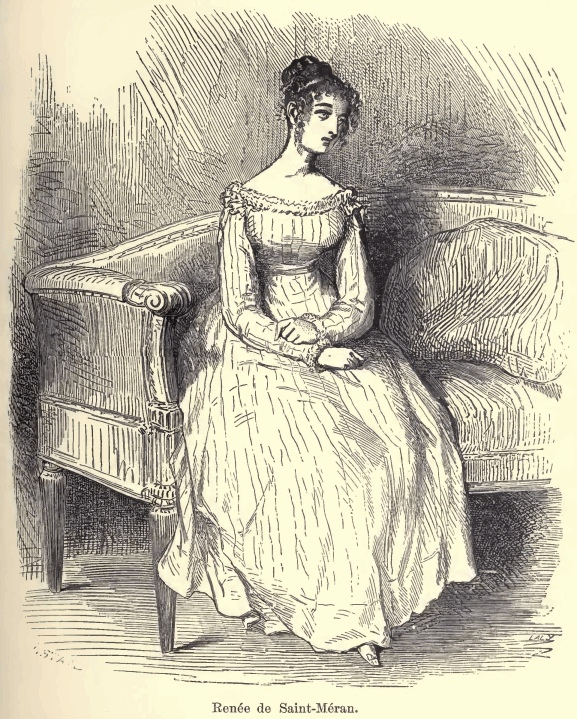
\includegraphics[width=\textwidth]{0091m.jpg}
\end{figure}

“That is true,” answered the marquis.

“How much do I owe this gracious prince! What is there I would not do
to evince my earnest gratitude!”

“That is right,” cried the marquise. “I love to see you thus. Now,
then, were a conspirator to fall into your hands, he would be most
welcome.”

“For my part, dear mother,” interposed Renée, “I trust your wishes will
not prosper, and that Providence will only permit petty offenders, poor
debtors, and miserable cheats to fall into M. de Villefort’s
hands,—then I shall be contented.”

“Just the same as though you prayed that a physician might only be
called upon to prescribe for headaches, measles, and the stings of
wasps, or any other slight affection of the epidermis. If you wish to
see me the king’s attorney, you must desire for me some of those
violent and dangerous diseases from the cure of which so much honor
redounds to the physician.”

At this moment, and as though the utterance of Villefort’s wish had
sufficed to effect its accomplishment, a servant entered the room, and
whispered a few words in his ear. Villefort immediately rose from table
and quitted the room upon the plea of urgent business; he soon,
however, returned, his whole face beaming with delight. Renée regarded
him with fond affection; and certainly his handsome features, lit up as
they then were with more than usual fire and animation, seemed formed
to excite the innocent admiration with which she gazed on her graceful
and intelligent lover.

“You were wishing just now,” said Villefort, addressing her, “that I
were a doctor instead of a lawyer. Well, I at least resemble the
disciples of Esculapius in one thing [people spoke in this style in
1815], that of not being able to call a day my own, not even that of my
betrothal.”

“And wherefore were you called away just now?” asked Mademoiselle de
Saint-Méran, with an air of deep interest.

“For a very serious matter, which bids fair to make work for the
executioner.”

“How dreadful!” exclaimed Renée, turning pale.

“Is it possible?” burst simultaneously from all who were near enough to
the magistrate to hear his words.

“Why, if my information prove correct, a sort of Bonapartist conspiracy
has just been discovered.”

“Can I believe my ears?” cried the marquise.

“I will read you the letter containing the accusation, at least,” said
Villefort:

“‘The king’s attorney is informed by a friend to the throne and the
religious institutions of his country, that one named Edmond Dantès,
mate of the ship \textit{Pharaon}, this day arrived from Smyrna, after having
touched at Naples and Porto-Ferrajo, has been the bearer of a letter
from Murat to the usurper, and again taken charge of another letter
from the usurper to the Bonapartist club in Paris. Ample corroboration
of this statement may be obtained by arresting the above-mentioned
Edmond Dantès, who either carries the letter for Paris about with him,
or has it at his father’s abode. Should it not be found in the
possession of father or son, then it will assuredly be discovered in
the cabin belonging to the said Dantès on board the \textit{Pharaon}.’”

“But,” said Renée, “this letter, which, after all, is but an anonymous
scrawl, is not even addressed to you, but to the king’s attorney.”

\begin{figure}[ht]
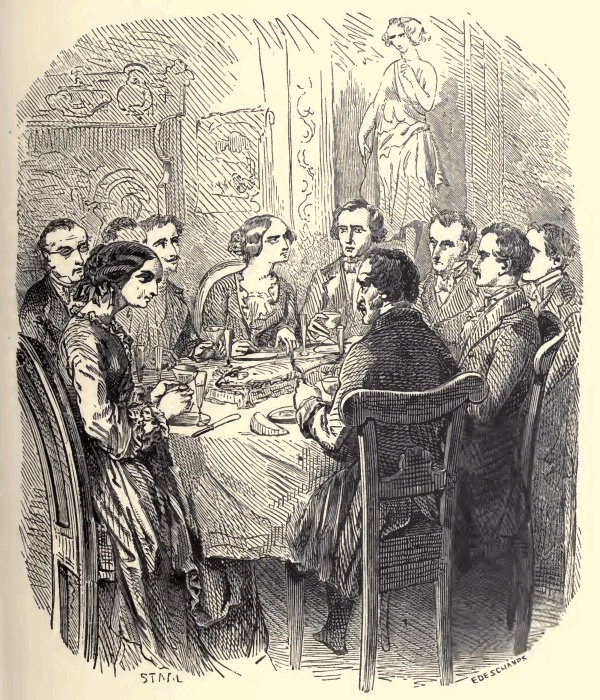
\includegraphics[width=\textwidth]{0093m.jpg}
\end{figure}

“True; but that gentleman being absent, his secretary, by his orders,
opened his letters; thinking this one of importance, he sent for me,
but not finding me, took upon himself to give the necessary orders for
arresting the accused party.”

“Then the guilty person is absolutely in custody?” said the marquise.

“Nay, dear mother, say the accused person. You know we cannot yet
pronounce him guilty.”

“He is in safe custody,” answered Villefort; “and rely upon it, if the
letter is found, he will not be likely to be trusted abroad again,
unless he goes forth under the especial protection of the headsman.”

“And where is the unfortunate being?” asked Renée.

“He is at my house.”

“Come, come, my friend,” interrupted the marquise, “do not neglect your
duty to linger with us. You are the king’s servant, and must go
wherever that service calls you.”

“Oh, Villefort!” cried Renée, clasping her hands, and looking towards
her lover with piteous earnestness, “be merciful on this the day of our
betrothal.”

The young man passed round to the side of the table where the fair
pleader sat, and leaning over her chair said tenderly:

“To give you pleasure, my sweet Renée, I promise to show all the lenity
in my power; but if the charges brought against this Bonapartist hero
prove correct, why, then, you really must give me leave to order his
head to be cut off.”

Renée shuddered at the word \textit{cut}, for the growth in question had a
head.

“Never mind that foolish girl, Villefort,” said the marquise. “She will
soon get over these things.” So saying, Madame de Saint-Méran extended
her dry bony hand to Villefort, who, while imprinting a son-in-law’s
respectful salute on it, looked at Renée, as much as to say, “I must
try and fancy ’tis your dear hand I kiss, as it should have been.”

“These are mournful auspices to accompany a betrothal,” sighed poor
Renée.

“Upon my word, child!” exclaimed the angry marquise, “your folly
exceeds all bounds. I should be glad to know what connection there can
possibly be between your sickly sentimentality and the affairs of the
state!”

“Oh, mother!” murmured Renée.

“Nay, madame, I pray you pardon this little traitor. I promise you that
to make up for her want of loyalty, I will be most inflexibly severe;”
then casting an expressive glance at his betrothed, which seemed to
say, “Fear not, for your dear sake my justice shall be tempered with
mercy,” and receiving a sweet and approving smile in return, Villefort
departed with paradise in his heart.
